\chapter{Non-Standard Evaluation}\label{nse}

The biggest difference between R and Python is not where R starts counting,
but its use of \gref{g:lazy-evaluation}{lazy evaluation}.
Nothing in R truly makes sense until we understand how this works.
Our discussion is more technical than some,
as it assumes the reader understands what a \gref{g:call-stack}{call stack} is
and is willing to expand their consciousness in hitherto unimaginable ways.

\section{How does Python evaluate function calls?}

Let's start by looking at a small Python program and its output:

\begin{lstlisting}
def ones_func(ones_arg):
    return ones_arg + " ones"

def tens_func(tens_arg):
    return ones_func(tens_arg + " tens")

initial = "start"
final = tens_func(initial + " more")
print(final)
\end{lstlisting}

\begin{lstlisting}
start more tens ones
\end{lstlisting}

When we call \texttt{tens\_func} we pass it \texttt{initial + " more"}.
Since \texttt{initial} has just been assigned the value \texttt{"start"},
that is the same as calling \texttt{tens\_func} with \texttt{"start more"}.
\texttt{tens\_func} then calls \texttt{ones\_func} with \texttt{"start more tens"},
and \texttt{ones\_func} returns \texttt{"start more tens ones"}.

But more is going on here than this three-sentence summary suggests.
Let's spell out the steps:

\begin{lstlisting}
def ones_func(ones_arg):
    ones_temp_1 = ones_arg + " ones"
    return ones_temp_1

def tens_func(tens_arg):
    tens_temp_1 = tens_arg + " tens"
    tens_temp_2 = ones_func(tens_temp_1)
    return tens_temp_2

initial = "start"
global_temp_1 = initial + " more"
final = tens_func(global_temp_1)
print(final)
\end{lstlisting}

\begin{lstlisting}
start more tens ones
\end{lstlisting}

{\sc FIXME: I would like to set these diagrams and steps in two columns,
  but (a) there isn't width and (b) I don't know your preferred way of doing that.
  I also need to rework some of the diagrams:
  some HTML tags seem to appear as text in the ones shown below
  for reasons I don't understand.}

Step 1: we assign \texttt{"start"} to \texttt{initial} at the global level
(Figure~\ref{fig:py-step-1}).

\begin{figure}[h]
  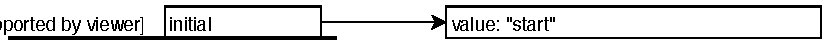
\includegraphics{figures/nse/python-step-01.pdf}
  \caption{Python Step 1}
  \label{fig:py-step-1}
\end{figure}

Step 2: we ask Python to call \texttt{tens\_func(initial + "more")},
so it creates a temporary variable to hold the result of the concatenation
\emph{before} calling \texttt{tens\_func}
(Figure~\ref{fig:py-step-2}).

\begin{figure}[h]
  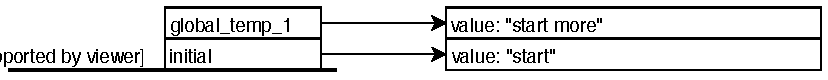
\includegraphics{figures/nse/python-step-02.pdf}
  \caption{Python Step 2}
  \label{fig:py-step-2}
\end{figure}

Step 3: Python creates a new stack frame to hold the call to \texttt{tens\_func}
(Figure~\ref{fig:py-step-3}).
Note that \texttt{tens\_arg} points to the same thing in memory as \texttt{global\_temp\_1},
since Python passes everything by reference.

\begin{figure}[h]
  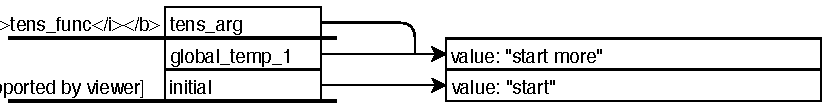
\includegraphics{figures/nse/python-step-03.pdf}
  \caption{Python Step 3}
  \label{fig:py-step-3}
\end{figure}

Step 4: we ask Python to call \texttt{ones\_func(tens\_arg + " tens")},
so it creates another temporary variable
(Figure~\ref{fig:py-step-4}).

\begin{figure}[h]
  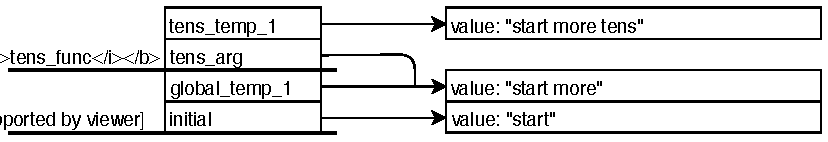
\includegraphics{figures/nse/python-step-04.pdf}
  \caption{Python Step 4}
  \label{fig:py-step-4}
\end{figure}

Step 5: Python creates a new stack frame to manage the call to \texttt{ones\_func}
(Figure~\ref{fig:py-step-5}).

\begin{figure}[h]
  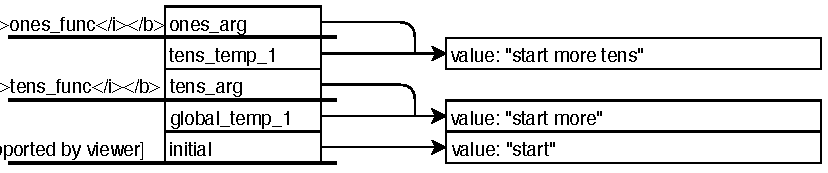
\includegraphics{figures/nse/python-step-05.pdf}
  \caption{Python Step 5}
  \label{fig:py-step-5}
\end{figure}

Step 6: Python creates a temporary variable to hold \texttt{ones\_arg + "ones"}
(Figure~\ref{fig:py-step-6}).

\begin{figure}[h]
  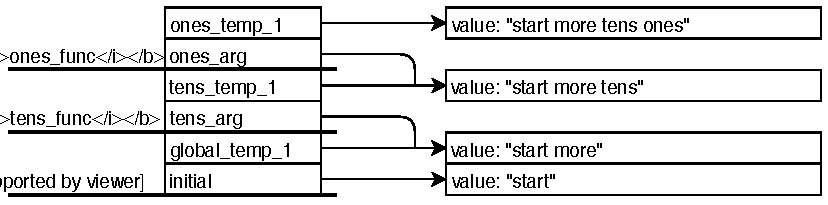
\includegraphics{figures/nse/python-step-06.pdf}
  \caption{Python Step 6}
  \label{fig:py-step-6}
\end{figure}

Step 7: Python returns from \texttt{ones\_func}
and puts its result in yet another temporary variable in \texttt{tens\_func}
(Figure~\ref{fig:py-step-7}).

\begin{figure}[h]
  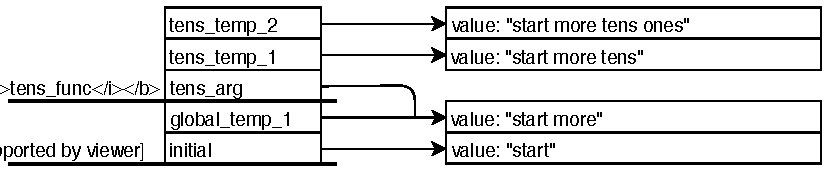
\includegraphics{figures/nse/python-step-07.pdf}
  \caption{Python Step 7}
  \label{fig:py-step-7}
\end{figure}

Step 8: Python returns from \texttt{tens\_func}
and puts that call's result in \texttt{final}
(Figure~\ref{fig:py-step-8}).

\begin{figure}[h]
  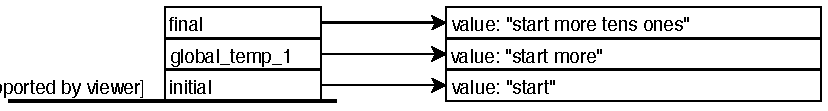
\includegraphics{figures/nse/python-step-08.pdf}
  \caption{Python Step 8}
  \label{fig:py-step-8}
\end{figure}

The most important thing here is that
Python evaluates expressions \emph{before} it calls functions,
and passes the results of those evaluations to the functions.
This is called \gref{g:eager-evaluation}{eager evaluation},
and is what most widely-used programming languages do.

\section{How does R evaluate function calls?}

In contrast,
R uses \gref{g:lazy-evaluation}{lazy evaluation}:
it doesn't evaluate the arguments to a function until their values are needed,
which is usually \emph{after} the function has been called.
To illustrate,
here's an R program equivalent to the Python shown above:

\begin{lstlisting}
ones_func <- function(ones_arg) {
  paste(ones_arg, "ones")
}

tens_func <- function(tens_arg) {
  ones_func(paste(tens_arg, "tens"))
}

initial <- "start"
final <- tens_func(paste(initial, "more"))
print(final)
\end{lstlisting}

\begin{lstlisting}
[1] "start more tens ones"
\end{lstlisting}

And here it is with the intermediate steps spelled out in a syntax we just made up:

\begin{lstlisting}
ones_func <- function(ones_arg) {
  ones_arg.RESOLVE(@tens_func@, paste(tens_arg, "tens"), "start more tens")
  ones_temp_1 <- paste(ones_arg, "ones")
  return(ones_temp_1)
}

tens_func <- function(tens_arg) {
  tens_arg.RESOLVE(@global@, paste(initial, "more"), "start more")
  tens_temp_1 <- PROMISE(@tens_func@, paste(tens_arg, "tens"), ____)
  tens_temp_2 <- ones_func(paste(tens_temp_1))
  return(tens_temp_2)
}

initial <- "start"
global_temp_1 <- PROMISE(@global@, paste(initial, "more"), ____)
final <- tens_func(global_temp_1)
print(final)
\end{lstlisting}

While the original code looked much like our Python,
the evaluation trace is very different,
and hinges on the fact that
\emph{an expression in a programming language can be represented as a data structure}.

\begin{quote}
\textbf{What's an Expression?}

An expression is anything that has a value.
The simplest expressions are literal values like the number 1,
the string \texttt{"stuff"}, and the Boolean \texttt{TRUE}.
A variable like \texttt{least} is also an expression:
its value is whatever the variable currently refers to.

Complex expressions are built out of simpler expressions:
\texttt{1 + 2} is an expression that uses \texttt{+} to combine 1 and 2,
while the expression \texttt{c(10, 20, 30)} uses the function \texttt{c}
to create a vector out of the values 10, 20, 30.
Expressions are often drawn as trees like this\footnote{
  ASCII art is not mandatory,
  but is the closest we can come to the carved runes used by our forebears.}:

\begin{lstlisting}
    +
   / \
  1   2
\end{lstlisting}

When Python (or R, or any other language) reads a program,
it parses the text and builds trees like the one shown above
to represent what the program is supposed to do.
Processing that data structure to find its value
is called \gref{g:evaluation}{evaluating} the expression.

Most modern languages allow us to build trees ourselves,
either by concatenating strings to create program text
and then parsing and evaluating the result:

\begin{lstlisting}
left <- '1'
right <- '2'
op <- '+'
combined <- paste(left, op, right)
tree <- parse(text = combined)
\end{lstlisting}

\noindent
or by calling functions.
The function-based approach is safer and more flexible;
see \citet{Wick2019} for details.
\end{quote}

So how does R evaluate our little program?
Step 1: we assign ``start'' to \texttt{initial} in the \gref{g:global-environment}{global environment}
(Figure~\ref{fig:r-step-1}).

\begin{figure}[h]
  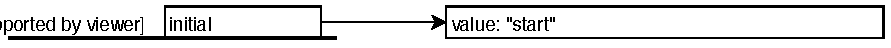
\includegraphics{figures/nse/r-step-01.pdf}
  \caption{R Step 1}
  \label{fig:r-step-1}
\end{figure}

Step 2: we ask R to call \texttt{tens\_func(initial + "more")}
(Figure~\ref{fig:r-step-2}).
To do this,
it creates a \gref{g:promise}{promise} to hold:

\begin{itemize}
\item
  the \gref{g:environment}{environment} we're in (which we are surrounding with \texttt{@}),
\item
  the expression we're passing to the function, and
\item
  the value of that expression (which we are showing as \texttt{\_\_\_\_}, since it's initially empty).
\end{itemize}

\begin{figure}[h]
  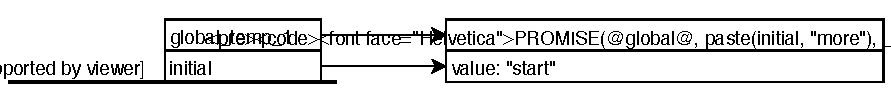
\includegraphics{figures/nse/r-step-02.pdf}
  \caption{R Step 2}
  \label{fig:r-step-2}
\end{figure}

In Step 3,
R passes that promise into \texttt{tens\_func}
(Figure~\ref{fig:r-step-3}).
Crucially,
the promise in \texttt{tens\_func} remembers that
it was created in the \gref{g:global-environment}{global environment}:
it will eventually need a value for \texttt{initial},
so it needs to know where to look to find the right one.

\begin{figure}[h]
  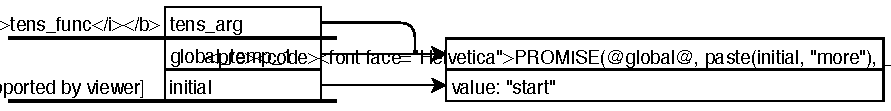
\includegraphics{figures/nse/r-step-03.pdf}
  \caption{R Step 3}
  \label{fig:r-step-3}
\end{figure}

Step 4: since the very next thing we ask for is \texttt{paste(tens\_arg, "tens")},
R needs a value for \texttt{tens\_arg}.
To get it,
R evaluates the promise that \texttt{tens\_arg} refers to
(Figure~\ref{fig:r-step-4}).
This evaluation happens \emph{after} \texttt{tens\_func} has been called,
not before as in Python,
which is why this scheme is called ``lazy'' evaluation.
Once a promise has been resolved,
R uses its value,
and that value never changes.

\begin{figure}[h]
  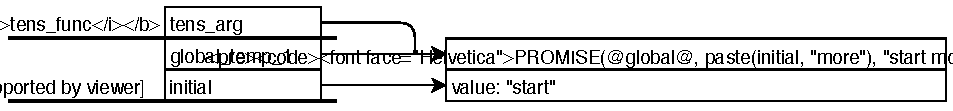
\includegraphics{figures/nse/r-step-04.pdf}
  \caption{R Step 4}
  \label{fig:r-step-4}
\end{figure}

Step 5:
\texttt{tens\_func} wants to call \texttt{ones\_func},
so R creates another promise to record what's being passed into \texttt{ones\_func}
(Figure~\ref{fig:r-step-5}).

\begin{figure}[h]
  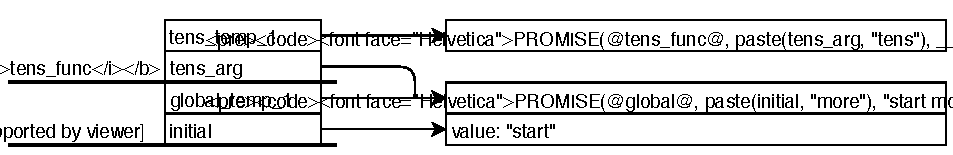
\includegraphics{figures/nse/r-step-05.pdf}
  \caption{R Step 5}
  \label{fig:r-step-5}
\end{figure}

Step 6:
R calls \texttt{ones\_func},
binding the newly-created promise to \texttt{ones\_arg} as it does so
(Figure~\ref{fig:r-step-6}).

\begin{figure}[h]
  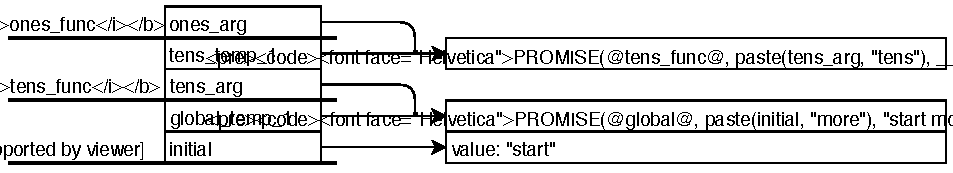
\includegraphics{figures/nse/r-step-06.pdf}
  \caption{R Step 6}
  \label{fig:r-step-6}
\end{figure}

Step 7:
R needs a value for \texttt{ones\_arg} to pass to \texttt{paste},
so it resolves the promise
(Figure~\ref{fig:r-step-7}).

\begin{figure}[h]
  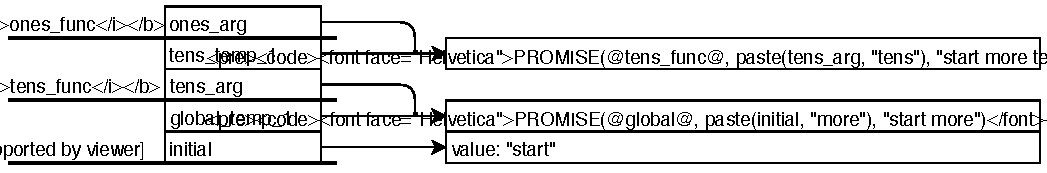
\includegraphics{figures/nse/r-step-07.pdf}
  \caption{R Step 7}
  \label{fig:r-step-7}
\end{figure}

Step 8: \texttt{ones\_func} uses \texttt{paste} to concatenate strings
(Figure~\ref{fig:r-step-8}).

\begin{figure}[h]
  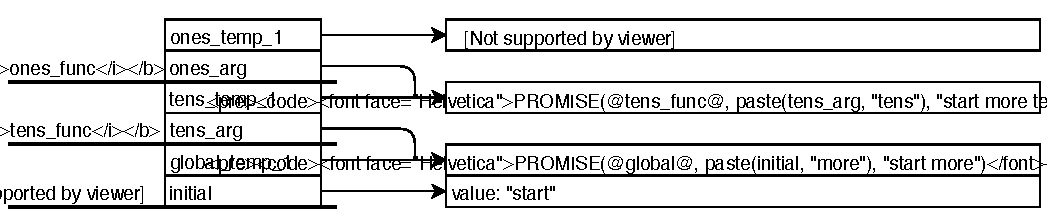
\includegraphics{figures/nse/r-step-08.pdf}
  \caption{R Step 8}
  \label{fig:r-step-8}
\end{figure}

Steps 9 and 10:
\texttt{ones\_func} and \texttt{tens\_func} return
(Figures~\ref{fig:r-step-9} and~\ref{fig:r-step-10}).

\begin{figure}[h]
  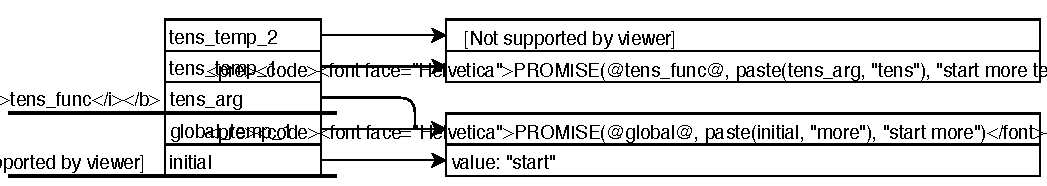
\includegraphics{figures/nse/r-step-09.pdf}
  \caption{R Step 9}
  \label{fig:r-step-9}
\end{figure}

\begin{figure}[h]
  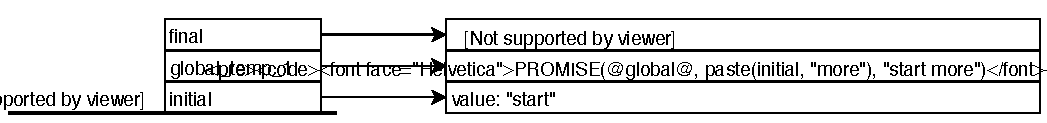
\includegraphics{figures/nse/r-step-10.pdf}
  \caption{R Step 10}
  \label{fig:r-step-10}
\end{figure}

We got the same answer as we did in Python,
but in a significantly different way.
Each time we passed something into a function,
R created a promise to record what it was and where it came from,
and then resolved the promise when the value was needed.

R \emph{always} does this---if we call:

\begin{lstlisting}
sign(2)
\end{lstlisting}

\noindent
then behind the scenes,
R is creating a promise and passing it to \texttt{sign},
where it is automatically resolved to get the number 2 when its value is needed.
(If we wanted to be thorough,
we would have shown the promises passed into \texttt{paste} at each stage of execution above.)

\section{Why is lazy evaluation useful?}

Lazy evaluation would be pointless if it always produced the same answer as eager evaluation,
but it doesn't have to.
To see how powerful lazy evaluation can be,
let's create an expression of our own:

\begin{lstlisting}
my_expr <- expr(red)
\end{lstlisting}

\noindent
Displaying the value of \texttt{my\_expr} isn't very exciting:

\begin{lstlisting}
my_expr
\end{lstlisting}

\begin{lstlisting}
red
\end{lstlisting}

\noindent
but what kind of thing is it?

\begin{lstlisting}
typeof(my_expr)
\end{lstlisting}

\begin{lstlisting}
[1] "symbol"
\end{lstlisting}

A symbol is a kind of expression.
It is not a string,
though strings can be converted to symbols and symbols to strings.
Nor is it a value: yet.
If we try to get the value it refers to, R displays an error message:

\begin{lstlisting}
eval(my_expr)
\end{lstlisting}

\begin{lstlisting}
Error in eval(my_expr): object 'red' not found
\end{lstlisting}

\noindent
We haven't created a variable called \texttt{red},
so R cannot evaluate an expression that asks for it.

But what if we create such a variable now and then re-evaluate the expression?

\begin{lstlisting}
red <- "this is red"
eval(my_expr)
\end{lstlisting}

\begin{lstlisting}
[1] "this is red"
\end{lstlisting}

\noindent
More usefully,
what if we create something that has a value for \texttt{red}:

\begin{lstlisting}
color_data <- tribble(
  ~red, ~green,
     1,     10,
     2,     20
)
color_data
\end{lstlisting}

\begin{lstlisting}
# A tibble: 2 x 2
    red green
  <dbl> <dbl>
1     1    10
2     2    20
\end{lstlisting}

\noindent
and then ask R to evaluate our expression in the \gref{g:context}{context} of that tibble:

\begin{lstlisting}
eval(my_expr, color_data)
\end{lstlisting}

\begin{lstlisting}
[1] 1 2
\end{lstlisting}

When we call \texttt{eval},
it looks for definitions of variables in the data structure we've given it---in this case,
the tibble \texttt{color\_data}.
Since that tibble has a column called \texttt{red},
\texttt{eval(my\_expr, color\_data)} gives us that column.

This may not seem life-changing yet,
but being able to pass expressions around
and evaluate them in contexts of our choosing allows us to seem very clever indeed.
For example,
let's create another expression:

\begin{lstlisting}
add_red_green <- expr(red + green)
typeof(add_red_green)
\end{lstlisting}

\begin{lstlisting}
[1] "language"
\end{lstlisting}

The type of \texttt{add\_red\_green} is \texttt{language} rather than \texttt{symbol}
because it contains more than just a single symbol.
It is still an expression,
though,
so we can evaluate it in the context of our data frame:

\begin{lstlisting}
eval(add_red_green, color_data)
\end{lstlisting}

\begin{lstlisting}
[1] 11 22
\end{lstlisting}

Still not convinced?
Have a look at this function:

\begin{lstlisting}
run_many_checks <- function(data, ...) {
  conditions <- list(...)
  checks <- vector("list", length(conditions))
  for (i in seq_along(conditions)) {
    checks[[i]] <- eval(conditions[[i]], data)
  }
  checks
}
\end{lstlisting}

\noindent
\texttt{run\_many\_checks} takes a tibble and some logical expressions,
evaluates each expression in turn,
and returns a list of results:

\begin{lstlisting}
run_many_checks(color_data, expr(0 < red), expr(red < green))
\end{lstlisting}

\begin{lstlisting}
[[1]]
[1] TRUE TRUE

[[2]]
[1] TRUE TRUE
\end{lstlisting}

We can take it one step further
and simply report whether all the checks passed or not:

\begin{lstlisting}
run_all_checks <- function(data, ...) {
  conditions <- list(...)
  checks <- vector("logical", length(conditions))
  for (i in seq_along(conditions)) {
    checks[[i]] <- all(eval(conditions[[i]], data))
  }
  all(checks)
}

run_all_checks(color_data, expr(0 < red), expr(red < green))
\end{lstlisting}

\begin{lstlisting}
[1] TRUE
\end{lstlisting}

This is cool,
but typing \texttt{expr(...)} over and over feels clumsy.
It also seems superfluous,
since we know that arguments aren't evaluated before they're passed into functions.
Can we get rid of this and write something that does this?

\begin{lstlisting}
run_all_checks(color_data, 0 < red, red < green)
\end{lstlisting}

\noindent
The answer is going to be ``yes'',
but it's going to take a bit of work.

\begin{quote}
\textbf{Square Brackets{\ldots} Why'd It Have to Be Square Brackets?}

Before we go there,
a word (or code snippet) of warning.
The first version of \texttt{run\_many\_checks} essentially did this:

\begin{lstlisting}
conditions <- list(expr(red < green))
eval(conditions[1], color_data)
\end{lstlisting}

\noindent
What we did wrong was use \texttt{[} instead of \texttt{[[},
which meant that \texttt{conditions[1]} was not an expression---it was a list containing a single expression.
It turns out that evaluating a list containing an expression produces a list of expressions rather than an error,
which is so helpful that it only took me an hour to figure out my mistake.
\end{quote}

\section{What is tidy evaluation?}

Our goal is to write something that looks like it belongs in the tidyverse.
We want to be able to write this:

\begin{lstlisting}
check_all(color_data, 0 < red, red < green)
\end{lstlisting}

\noindent
without calling \texttt{expr} to quote our expressions explicitly.
For simplicity's sake,
our first attempt only handles a single expression:

\begin{lstlisting}
check_naive <- function(data, test) {
  eval(test, data)
}
\end{lstlisting}

\noindent
When we try it, it fails:

\begin{lstlisting}
check_naive(color_data, red != green)
\end{lstlisting}

\begin{lstlisting}
Error in eval(test, data): object 'green' not found
\end{lstlisting}

\noindent
This actually makes sense:
by the time we reach the call to \texttt{eval},
\texttt{test} refers to a promise that represents the value of \texttt{red != green} in the global environment.
Promises are not expressions---each promise contains an expression,
but it also contains an environment and a copy of the expression's value (if it has ever been calculated).
As a result,
when R sees the call to \texttt{eval} inside \texttt{check\_naive}
it automatically tries to resolve the promise that contains \texttt{left != right},
and fails because there are no variables with those names in the global environment.

So how can we get the expression out of the promise without triggering evaluation?
One way is to use a function called \texttt{substitute}:

\begin{lstlisting}
check_using_substitute <- function(data, test) {
  subst_test <- substitute(test)
  eval(subst_test, data)
}

check_using_substitute(color_data, red != green)
\end{lstlisting}

\begin{lstlisting}
[1] TRUE TRUE
\end{lstlisting}

\noindent
However,
\texttt{substitute} is frowned upon because it behaves one way when called interactively on the command line
and another way when called inside a function.
Instead,
we can use a function called \texttt{enquo} from the \texttt{rlang} package.
\texttt{enquo} returns an object called a \gref{g:quosure}{quosure}
that contains only an unevaluated expression and an environment:

\begin{lstlisting}
check_using_enquo <- function(data, test) {
  q_test <- enquo(test)
  eval(q_test, data)
}

check_using_enquo(color_data, red != green)
\end{lstlisting}

\begin{lstlisting}
<quosure>
expr: ^red != green
env:  global
\end{lstlisting}

\noindent
Ah: a quosure is a structured object,
so evaluating it just gives it back to us in the same way that evaluating \texttt{2} or \texttt{"hello"} would.
What we want to \texttt{eval} is the expression inside the quosure,
which we can get using \texttt{quo\_get\_expr}:

\begin{lstlisting}
check_using_quo_get_expr <- function(data, test) {
  q_test <- enquo(test)
  eval(quo_get_expr(q_test), data)
}

check_using_quo_get_expr(list(left = 1, right = 2), left != right)
\end{lstlisting}

\begin{lstlisting}
[1] TRUE
\end{lstlisting}

Enquoting and evaluating expressions is done so often in the tidyverse
that \texttt{rlang} provides a shortcut called \texttt{\{\{..\}\}}:

\begin{lstlisting}
max_of_var <- function(data, the_var) {
  data %>%
    group_by({{ the_var }}) %>%
    summarize(maximum = max({{ the_var }}))
}

max_of_var(color_data, red)
\end{lstlisting}

\begin{lstlisting}
# A tibble: 2 x 2
    red maximum
  <dbl>   <dbl>
1     1       1
2     2       2
\end{lstlisting}

We can use \texttt{\{\{..\}\}} to write a function \texttt{run\_two\_checks}
that runs two checks on some data:

\begin{lstlisting}
run_two_checks <- function(data, first_check, second_check) {
  first_result <- data %>%
    transmute(temp = {{ first_check }}) %>%
    pull(temp) %>%
    all()
  second_result <- data %>%
    transmute(temp = {{ second_check }})%>%
    pull(temp) %>% all()
  first_result && second_result
}

run_two_checks(color_data, 0 < red, red < green)
\end{lstlisting}

\begin{lstlisting}
[1] TRUE
\end{lstlisting}

That's much easier to follow than a bunch of \texttt{enquo} and \texttt{eval} calls,
but what if we want to handle an arbitrary number of checks?
Our first attempt is this:

\begin{lstlisting}
new_colors <- tribble(
  ~yellow, ~violet,
  1,       10,
  2,       20
)
run_all_checks <- function(data, ...) {
  conditions <- list(...)
  result = TRUE
  for (i in seq_along(conditions)) {
    cond = conditions[[i]]
    result <- result && data %>%
      transmute(temp = {{cond}}) %>%
      pull(temp) %>%
      all()
  }
  result
}

run_all_checks(new_colors, 0 < yellow, violet < yellow)
\end{lstlisting}

\begin{lstlisting}
Error in run_all_checks(new_colors, 0 < yellow, violet < yellow): object 'yellow' not found
\end{lstlisting}

This code fails because the call to \texttt{list(...)} tries to evaluate the expressions in \texttt{...}
when adding them to the list.
What we need to use instead is \texttt{enquos},
which does what \texttt{enquo} does but on \texttt{...}:

\begin{lstlisting}
run_all_checks <- function(data, ...) {
  conditions <- enquos(...)
  result = TRUE
  for (i in seq_along(conditions)) {
    cond = conditions[[i]]
    result <- result && data %>%
      transmute(temp = {{ cond }}) %>%
      pull(temp) %>%
      all()
  }
  result
}

run_all_checks(new_colors, 0 < yellow, violet < yellow)
\end{lstlisting}

\begin{lstlisting}
[1] FALSE
\end{lstlisting}

\section{What if we truly desire to venture into the depths?}

\texttt{\{\{..\}\}} and \texttt{enquos} will do almost everything we need from day to day,
but occasionally we may need to go one level deeper.
Our first exploration fails on purpose in order to demonstrate a common mistake:

\begin{lstlisting}
check_without_quoting_test <- function(data, test) {
  data %>%
    transmute(result = test) %>%
    pull(result) %>%
    all()
}
check_without_quoting_test(color_data, yellow < violet)
\end{lstlisting}

\begin{lstlisting}
Error: object 'yellow' not found
\end{lstlisting}

\noindent
It fails because we're not enquoting the test.
Let's modify it the code to enquote and then pass in the expression:

\begin{lstlisting}
check_without_quoting_test <- function(data, test) {
  q_test <- enquo(test)
  x_test <- quo_get_expr(q_test)
  data %>%
    transmute(result = x_test) %>%
    pull(result) %>%
    all()
}
check_without_quoting_test(new_colors, yellow < violet)
\end{lstlisting}

\begin{lstlisting}
Error: Column `result` is of unsupported type quoted call
\end{lstlisting}

Damn---we thought this one had a chance.
The problem is that when we say \texttt{result = x\_test},
what actually gets passed into \texttt{transmute} is a promise containing an expression.
Somehow,
we need to prevent R from doing that promise wrapping.

This brings us to \texttt{enquo}'s partner \texttt{!!},
which we can use to \gref{g:splice}{splice} the expression in a quosure into a function call.
\texttt{!!} is pronounced ``bang bang'' or ``oh hell'' depending on how your day is going.
It only works in contexts like function calls where R is automatically quoting things for us,
but if we use it then,
it does exactly what we want:

\begin{lstlisting}
check_using_bangbang <- function(data, test) {
  q_test <- enquo(test)
  data %>%
    transmute(result = !!q_test) %>%
    pull(result) %>%
    all()
}
check_using_bangbang(new_colors, yellow < violet)
\end{lstlisting}

\begin{lstlisting}
[1] TRUE
\end{lstlisting}

We are almost in a state of grace.
The two rules we must follow are:

\begin{enumerate}
\item
  Use \texttt{enquo} to enquote every argument that contains an unevaluated expression.
\item
  Use \texttt{!!} when passing each of those arguments into a tidyverse function.
\end{enumerate}

\begin{lstlisting}
check_all <- function(data, ...) {
  tests <- enquos(...)
  result <- TRUE
  for (t in tests) {
    result <- result && data %>%
      transmute(result = !!t) %>%
      pull(result) %>%
      all()
  }
  result
}

check_all(new_colors, 0 < yellow, yellow < violet)
\end{lstlisting}

\begin{lstlisting}
[1] TRUE
\end{lstlisting}

\noindent
And just to make sure that it fails when it's supposed to:

\begin{lstlisting}
check_all(new_colors, yellow == violet)
\end{lstlisting}

\begin{lstlisting}
[1] FALSE
\end{lstlisting}

Backing up a bit,
\texttt{!!} works because there are
\href{https://tidyeval.tidyverse.org/getting-up-to-speed.html\#whats-special-about-quoting-functions}{two kinds of functions in R}:
\gref{g:evaluating-function}{evaluating functions} and
\gref{g:quoting-function}{quoting functions}.
Evaluating functions take arguments as values---they're what most of us are used to working with---but
quoting functions aren't passed the values of expressions:
they are given the expressions themselves.
When we write \texttt{color\_data\$red},
the \texttt{\$} function is being passed \texttt{color\_data} and the quoted expression \texttt{red}.
This is why we can't use variables as field names with \texttt{\$}:

\begin{lstlisting}
the_string_red <- "red"
color_data$the_string_red
\end{lstlisting}

\begin{lstlisting}
Warning: Unknown or uninitialised column: 'the_string_red'.
\end{lstlisting}

\begin{lstlisting}
NULL
\end{lstlisting}

The square bracket operators \texttt{[} and \texttt{[[},
on the other hand,
are evaluating functions,
so we can give them a variable containing a column name and get either a single-column tibble:

\begin{lstlisting}
color_data[the_string_red]     # single square brackets
\end{lstlisting}

\begin{lstlisting}
# A tibble: 2 x 1
    red
  <dbl>
1     1
2     2
\end{lstlisting}

\noindent
or a naked vector:

\begin{lstlisting}
color_data[[the_string_red]]   # double square brackets
\end{lstlisting}

\begin{lstlisting}
[1] 1 2
\end{lstlisting}

\section{Is it worth it?}

Delayed evaluation and quoting are confusing for two reasons:

\begin{enumerate}
\item
  They expose machinery that most programmers have never had to deal with before (and might not even have known existed).
  It's rather like learning to drive an automatic transmission and then switching to a manual one---all of a sudden
  you have to worry about a gear shift and a clutch.
\item
  R's built-in tools don't behave as consistently as they could,
  and the core functions provided by the tidverse as alternatives use variations on a small number of names:
  \texttt{quo}, \texttt{quote}, and \texttt{enquo} might all appear on the same page.
\end{enumerate}

\noindent
That said,
being able to pass column names to functions without wrapping them in strings is very useful,
and many powerful tools (such as using formulas in models)
rely on taking unevaluated expressions apart and rearranging them.
If you would like to know more,
or check that what you now think you understand is accurate,
\href{https://ijlyttle.shinyapps.io/tidyeval/}{this tutorial} is a good next step.

\section{Key Points}

\begin{itemize}
\item
  R uses lazy evaluation: expressions are evaluated when their values are needed, not before.
\item
  Use \texttt{expr} to create an expression without evaluating it.
\item
  Use \texttt{eval} to evaluate an expression in the context of some data.
\item
  Use \texttt{enquo} to create a quosure containing an unevaluated expression and its environment.
\item
  Use \texttt{quo\_get\_expr} to get the expression out of a quosure.
\item
  Use \texttt{!!} to splice the expression in a quosure into a function call.
\end{itemize}

\section{Exercises}

\begin{enumerate}


\item
  Explain why the code below \emph{doesn't} halt with an error.

\begin{lstlisting}
always_pi <- function(something) {
  3.14159
}

always_pi(stop("This message does not appear."))
\end{lstlisting}

\item
  Draw diagrams to show the objects in memory
  after each line of code below is executed:

\begin{lstlisting}
color_data <- tribble(
  ~red, ~green,
     1,     10,
     2,     20
)

get_column <- function(data, what) {
  eval(what, data)
}

my_expr <- expr(red)

get_column(color_data, my_expr)
\end{lstlisting}

\item
  Modify \texttt{get\_column} in the example above so that
  the caller doesn't have to create an expression explicitly,
  i.e.,
  so that \texttt{get\_column(color\_data, red)} will do the right thing.

\item
  Write a function \texttt{check\_any}
  that checks whether any of the conditions given are true for a data frame.
  Crucially,
  \texttt{check\_any} returns as soon as it finds a true condition
  \emph{without} evaluating any of the other conditions,
  so that this code runs without an error:

\begin{lstlisting}
color_data <- tribble(
  ~red, ~green,
     1,     10,
     2,     20
)

check_any(color_data, red > 0, stop("this message should not appear"))
\end{lstlisting}

\end{enumerate}
